\documentclass[10pt]{beamer}


% colors
\usepackage{xcolor}
\definecolor{mydarkgray}{gray}{0.33}
\definecolor{myred}{rgb}{0.85, 0.30, 0.0}
\definecolor{myblue}{rgb}{0.01, 0.45, 0.70}
\definecolor{mylightgray}{gray}{0.5}
\definecolor{mylightestgray}{gray}{0.9}


% beamer options
\setbeamertemplate{caption}[numbered]
\setbeamertemplate{frametitle}[default][center]
\setbeamertemplate{itemize items}[circle]
\setbeamertemplate{itemize subitem}{$\circ$}

\setbeamercolor{title}{fg=myblue}
\setbeamercolor{titlelike}{fg=mydarkgray}
\setbeamercolor{frametitle}{fg=mydarkgray, bg=mylightestgray}
\setbeamercolor{framesubtitle}{fg=mylightgray}
\setbeamercolor{itemize item}{fg=mydarkgray}
\setbeamercolor{itemize subitem}{fg=mydarkgray}


% figures
\usepackage{graphicx}


% language
\usepackage[english]{babel}
\usepackage[utf8]{inputenc}
\usepackage[T1]{fontenc}
\usepackage{pgfplotstable}
\usepackage{anyfontsize}

\usepackage{biblatex}
\addbibresource{references/refs.bib}
\renewcommand*{\bibfont}{\scriptsize}
% titlepage
\author{Xiao Chen, Bosko Todorovic, Yannic Laube, Zhi Wang}

\title{Which of the G10 Currencies is the Riskiest to Hold for a Swiss Resident?}

\institute{University of Zurich}
\date{\today}

\begin{document}
% ---------------------------------------------------------------------------
\begin{frame}
\titlepage
\end{frame}
% ---------------------------------------------------------------------------
\begin{frame}
\frametitle{Table of Contents}
\tableofcontents
\end{frame}
% ---------------------------------------------------------------------------
\begin{frame}
\section{Introduction}
\frametitle{Introduction}
\framesubtitle{G10 currencies}
G10 currencies refer to the ten most heavily traded and liquid currencies in the world~\cite{bis2022report}: 

United States Dollar (USD), Euro (EUR), British Pound (GBP), Japanese Yen (JPY), Australian Dollar (AUD), New Zealand Dollar (NZD), Canadian Dollar (CAD), Swiss Franc (CHF), Norwegian Krone (NOK), and Swedish Krona (SEK).

\end{frame}
% ---------------------------------------------------------------------------
\begin{frame}
\frametitle{Introduction}
\framesubtitle{G10 currencies}
Risks arising from exchange rate fluctuations:
\begin{itemize}
    \item Asset value depreciation
    \item Increased transaction costs
    \item Financial market volatility affecting their investment portfolios
\end{itemize}
\end{frame}
% ---------------------------------------------------------------------------
\begin{frame}
\section{Literature Review}
\frametitle{Literature Review}
Relationship between exchange rate fluctuations, international trade, and cross-border investments:~\cite{AUBOIN_RUTA_2013}
\begin{itemize}
    \item Exchange rate volatility introduces uncertainties for exporters and importers.
    \item Companies may experience revenue shrinkage with sharp exchange rate fluctuations.
\end{itemize}
\end{frame}
% ---------------------------------------------------------------------------
\begin{frame}
\frametitle{Literature Review}
Persistent exchange rate changes influence strategic decisions:~\cite{riker2020review}
\begin{itemize}
    \item U.S. dollar appreciation often reduces USD-denominated cross-border banking flows.~\cite{dollar_exchange}
    \item Higher risks on countries and corporations heavily reliant on USD debt.~\cite{dollar_exchange}
\end{itemize}
\end{frame}
% ---------------------------------------------------------------------------
\begin{frame}
\frametitle{Literature Review}
\framesubtitle{Characteristics}
\textbf{Liquidity}~\cite{rogoff2000six}
\begin{itemize}
    \item High foreign exchange trading volume
    \item Active derivatives trading
    \item Core position in foreign exchange reserves
\end{itemize}
\textbf{Stability}~\cite{campbell2002strategic}~\cite{engel2016exchange}
\begin{itemize}
    \item Strong economic foundations
    \item Safe-haven attributes
    \item Mitigate likelihood of extreme losses
\end{itemize}
\end{frame}
% ---------------------------------------------------------------------------
\begin{frame}
\frametitle{Literature Review}
\framesubtitle{Why Are G10 Currencies Important to Swiss Residents?}
\textbf{Trading and Investment}
\begin{itemize}
    \item Ease of Cross-Border Investment~\cite{rogoff2000six}: High-liquidity G10 currencies make it easier for Swiss residents to participate in global investment opportunities.
    \item Predictable Investment Returns~\cite{campbell2002strategic}~\cite{engel2016exchange}: Stable G10 currencies reduce exchange rate risks, making investment returns more predictable.
\end{itemize}
\end{frame}
% ---------------------------------------------------------------------------
\begin{frame}
\frametitle{Literature Review}
\framesubtitle{Why Are G10 Currencies Important to Swiss Residents?}
\textbf{Saving and Payments}
\begin{itemize}
    \item Euro as a Key Currency: Switzerland is near the Euro Area, so the euro (EUR) as the second main currency for Swiss residents is widely used for cross-border shopping, travel, and international payments~\cite{sif_imf_reports}.
\end{itemize}
\end{frame}
% ---------------------------------------------------------------------------
\begin{frame}
\frametitle{Literature Review}
\framesubtitle{Why Are G10 Currencies Important to Swiss Residents?}
\textbf{Asset Diversification and Safe-Haven Properties}   
\begin{itemize}
    \item Asset Diversification: The stability and liquidity of G10 currencies allow Swiss residents to diversify their assets. ~\cite{ito2020currency}
    \item Safe-Haven Currencies: Stable currencies show strong safe haven characteristics during periods of global financial turbulence or geopolitical instability.~\cite{ranaldo2010safe}
\end{itemize}
\end{frame}
% ---------------------------------------------------------------------------
\begin{frame}
\frametitle{Research Objective}
Compare and analyze: "Which of the G10 currencies is the riskiest to hold for a Swiss resident?"
\end{frame}
% ---------------------------------------------------------------------------
\begin{frame}
\section{Methodology}
\frametitle{Methodology}
The methods used include the calculation of \textbf{Expected Shortfall (ES)}, \textbf{Value-at-Risk (VaR)} through different models, the analysis of \textbf{volatilities}, and the investigation of the sensitivity of \textbf{exchange rate returns to interest rate} differentials.
\end{frame}
% ---------------------------------------------------------------------------
\begin{frame}
\frametitle{Methodology}
\framesubtitle{Expected Shortfall}

\end{frame}
% ---------------------------------------------------------------------------
\begin{frame}
\frametitle{Methodology}
\framesubtitle{Value-at-Risk (VaR)}
The loss that will not be exceeded with a certain probability and within a specified time period. 

Two different methods for calculating VaR were applied:
\begin{itemize}
    \item Historical calculation: Frequency = Month, $\alpha = 0.05$. 
    \item Monte Carlo simulation: Frequency = Day, $\alpha = 0.05$.
\end{itemize}.

\end{frame}
% ---------------------------------------------------------------------------
\begin{frame}
\frametitle{Methodology}
\framesubtitle{Historical vs. Monte Carlo Simulation}
\begin{itemize}
    \item \textbf{Historical calculation:} reflects realistic market conditions.
    \item \textbf{Monte Carlo simulation:} 10 simulations were conducted. The VaR for the simulated price paths and simulated returns was calculated for the last period of the simulation.x
\end{itemize}
\end{frame}
% ---------------------------------------------------------------------------
\begin{frame}
\frametitle{Methodology}
\framesubtitle{Volatility Analysis}
\begin{itemize}
    \item As a measure of the fluctuation intensity of the exchange rates, based on the standard deviation of the daily returns.
    \item The volatilities of the G10 currencies were compared to identify which currency poses the greatest risk for a Swiss investor.
    \item Time series plots were created to visualize volatility trends during the study period.
\end{itemize}
\end{frame}
% ---------------------------------------------------------------------------
\begin{frame}
\frametitle{Methodology}
\framesubtitle{Interest Rate Differentials Regression}
\begin{itemize}
    \item The sensitivity of exchange rate returns to interest rate differentials was examined by linear regression analysis. 
    \item Regression model: \[
    \text{log\_return}_{\text{exchange}} = \alpha + \beta \cdot \text{log\_diff}_{\text{interest\_rate}} + \epsilon
    \]
    \item Significance tests and confidence intervals were used to assess the statistical significance of the parameters.
\end{itemize}
\end{frame}
% ---------------------------------------------------------------------------
\begin{frame}
\section{Data}
\frametitle{Data}
\framesubtitle{Monthly Overnight Interest Rates}
\begin{itemize}
    \item From January 2000 to October 2024
    \item Data for G10 currencies (except Switzerland and Sweden) countries were obtained from the Federal Reserve Economic Data (FRED) database.
    \item Data for Switzerland was retrieved from the Swiss National Bank's (SNB) official API.
    \item Data for Sweden was sourced from the Swedish Riksbank’s Interest Rates and Exchange Rates Statistics.
\end{itemize}
\end{frame}
% ---------------------------------------------------------------------------
\begin{frame}
\frametitle{Data}
\framesubtitle{Daily Foreign Exchange Rates}
\begin{itemize}
    \item From January 1, 2004, to October 21, 2024
    \item Data for G10 currencies against the Swiss Franc (CHF) were collected using the YFinance library. 
\end{itemize}
\end{frame}
% ---------------------------------------------------------------------------
\begin{frame}
\section{Main Findings}
\frametitle{Main Findings}
\framesubtitle{Basic Risk Measures}

\end{frame}
% ---------------------------------------------------------------------------
\begin{frame}
\frametitle{Main Findings}
\framesubtitle{VaR Calculation}
In the historical VaR analysis, AUDCHF, CADCHF, NOKCHF, and NZDCHF all showed losses exceeding 1\%. 
\begin{table}[h]
\centering
\caption{\footnotesize Historical VaR (5\%) and Monte Carlo VaR (5\%) for each currency pair.} 
\label{tab:var_results}
\scalebox{0.48}{
    \pgfplotstabletypeset[
        col sep=comma,
        fixed zerofill,
        columns/Currency Pair/.style={string type},
        columns/Historical VaR/.style={
            fixed,
            precision=6,
            zerofill
        },
        columns/Monte Carlo VaR/.style={
            fixed,
            precision=6,
            zerofill
        },
        every head row/.style={before row=\hline, after row=\hline},
        every last row/.style={after row=\hline},
    ]{reports/figures/VaR_results.csv}
}
\end{table}
\begin{figure}[h]
    \centering   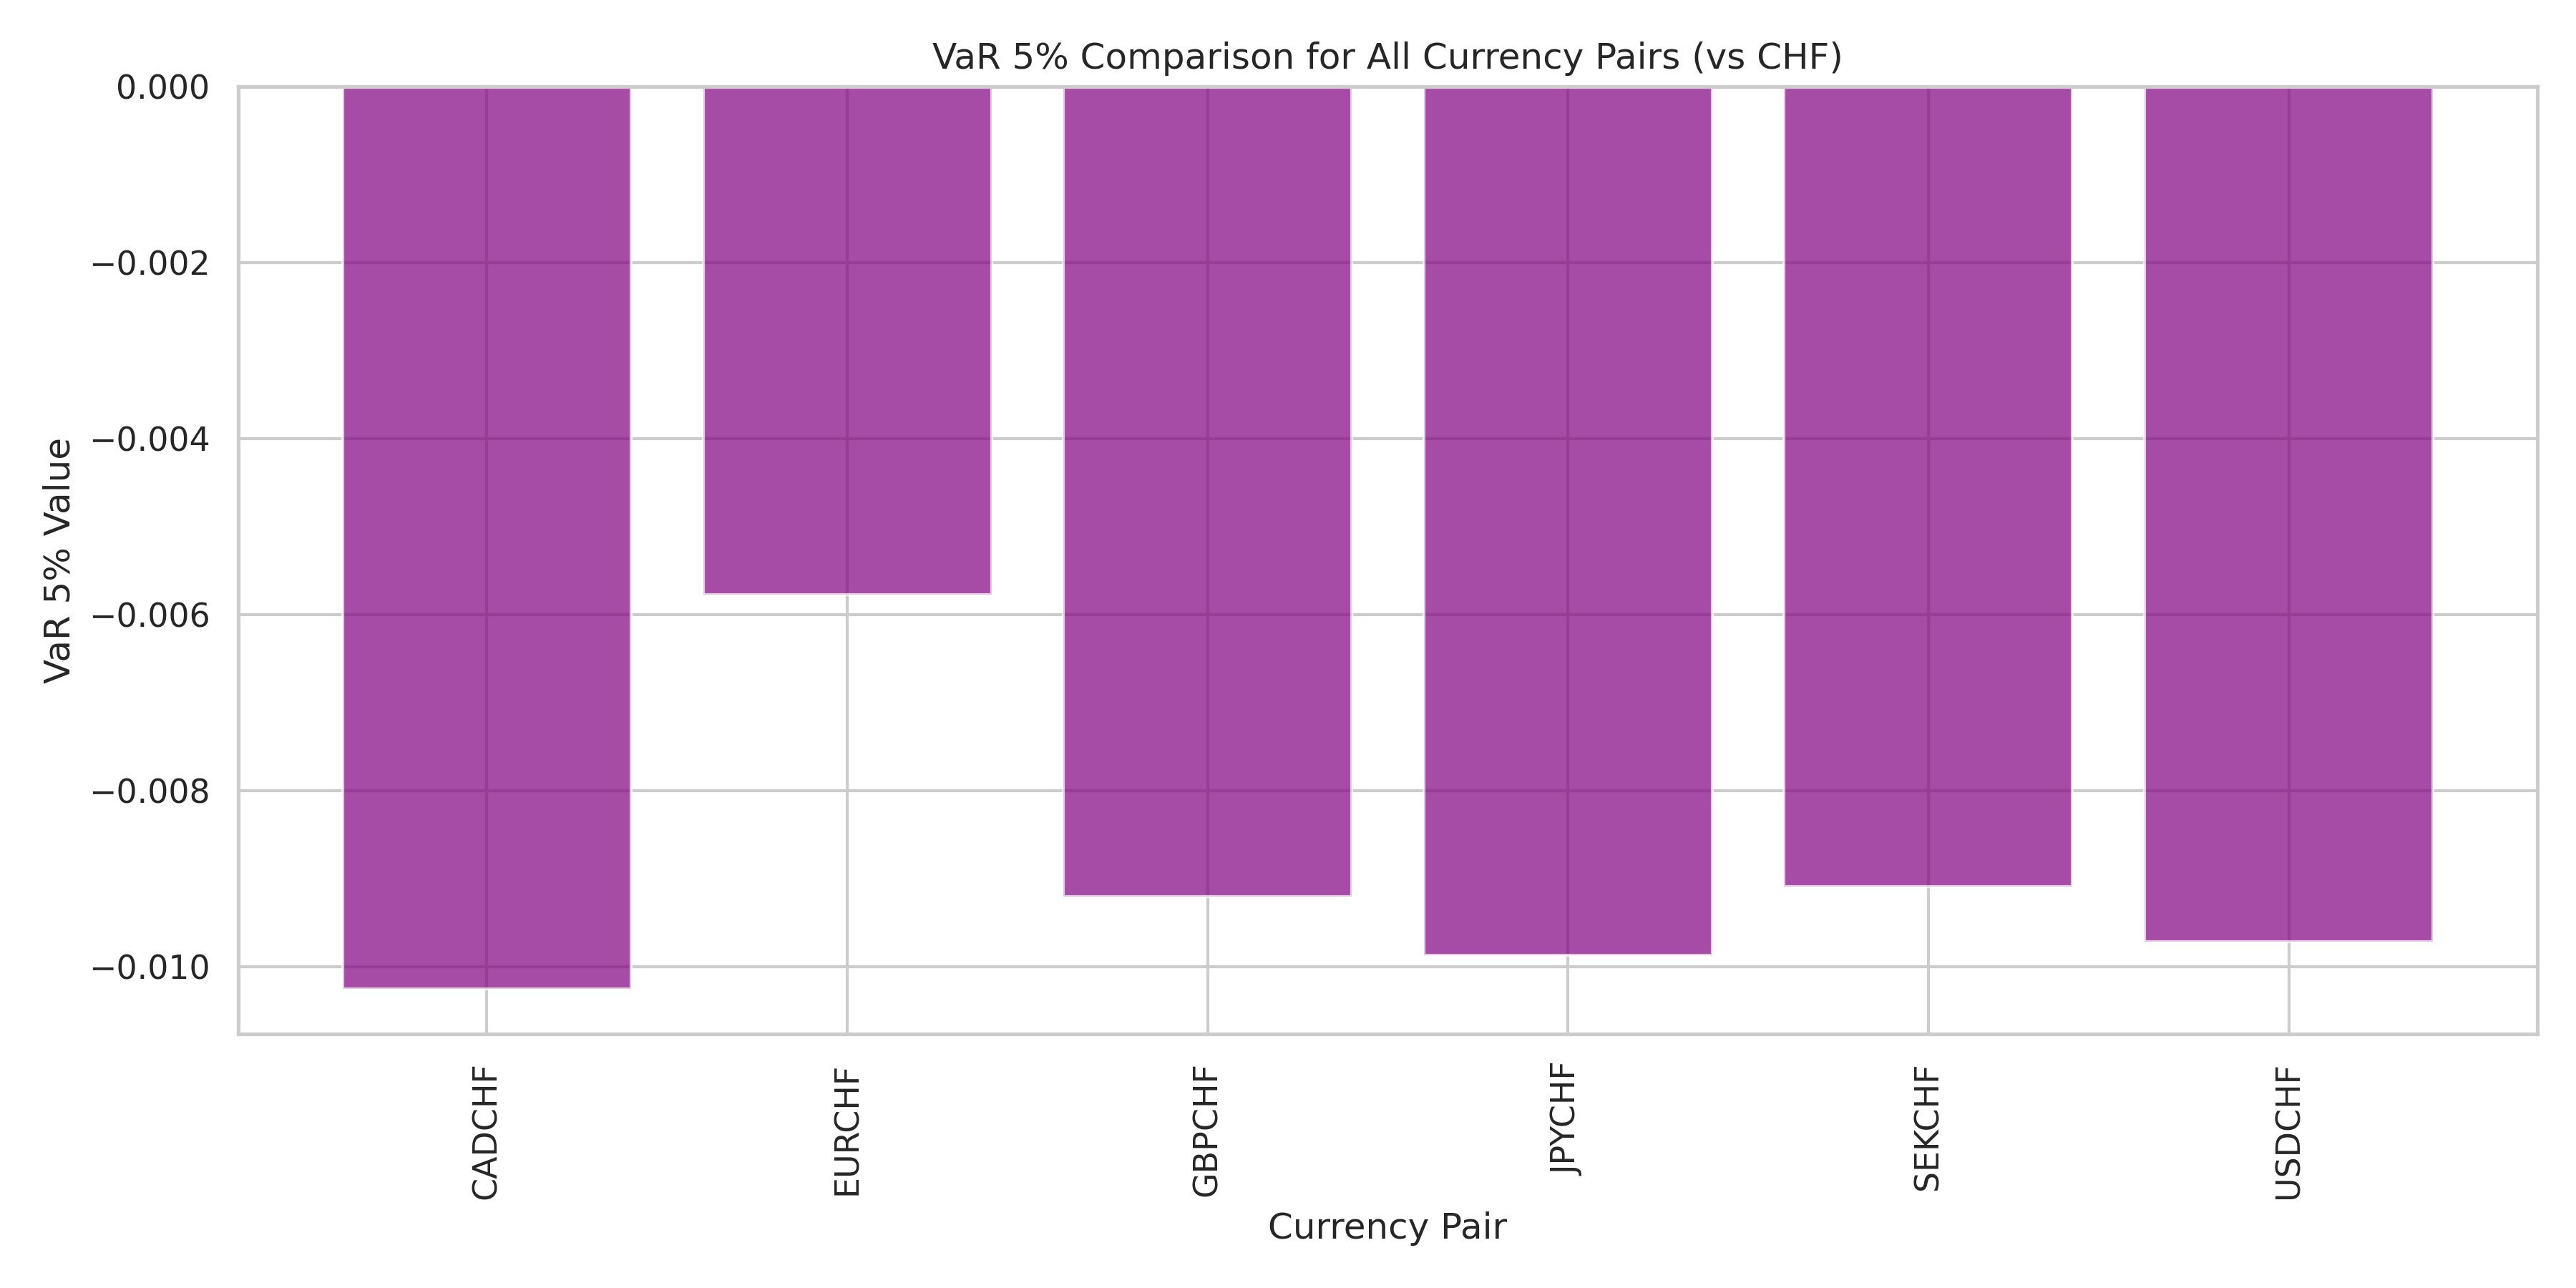
\includegraphics[width=0.48\linewidth]{reports/figures/var_5_percent_comparison_plot.png}
    \caption{\footnotesize Historical VaR of G10 currencies.}
    \label{fig:historical_VaR}
\end{figure}
\end{frame}
% ---------------------------------------------------------------------------
\begin{frame}
\frametitle{Main Findings}
\framesubtitle{VaR Calculation}
In the Monte Carlo simulation, AUD and NZD still exhibit high risk persistence.

\begin{figure}[h]
    \centering   
    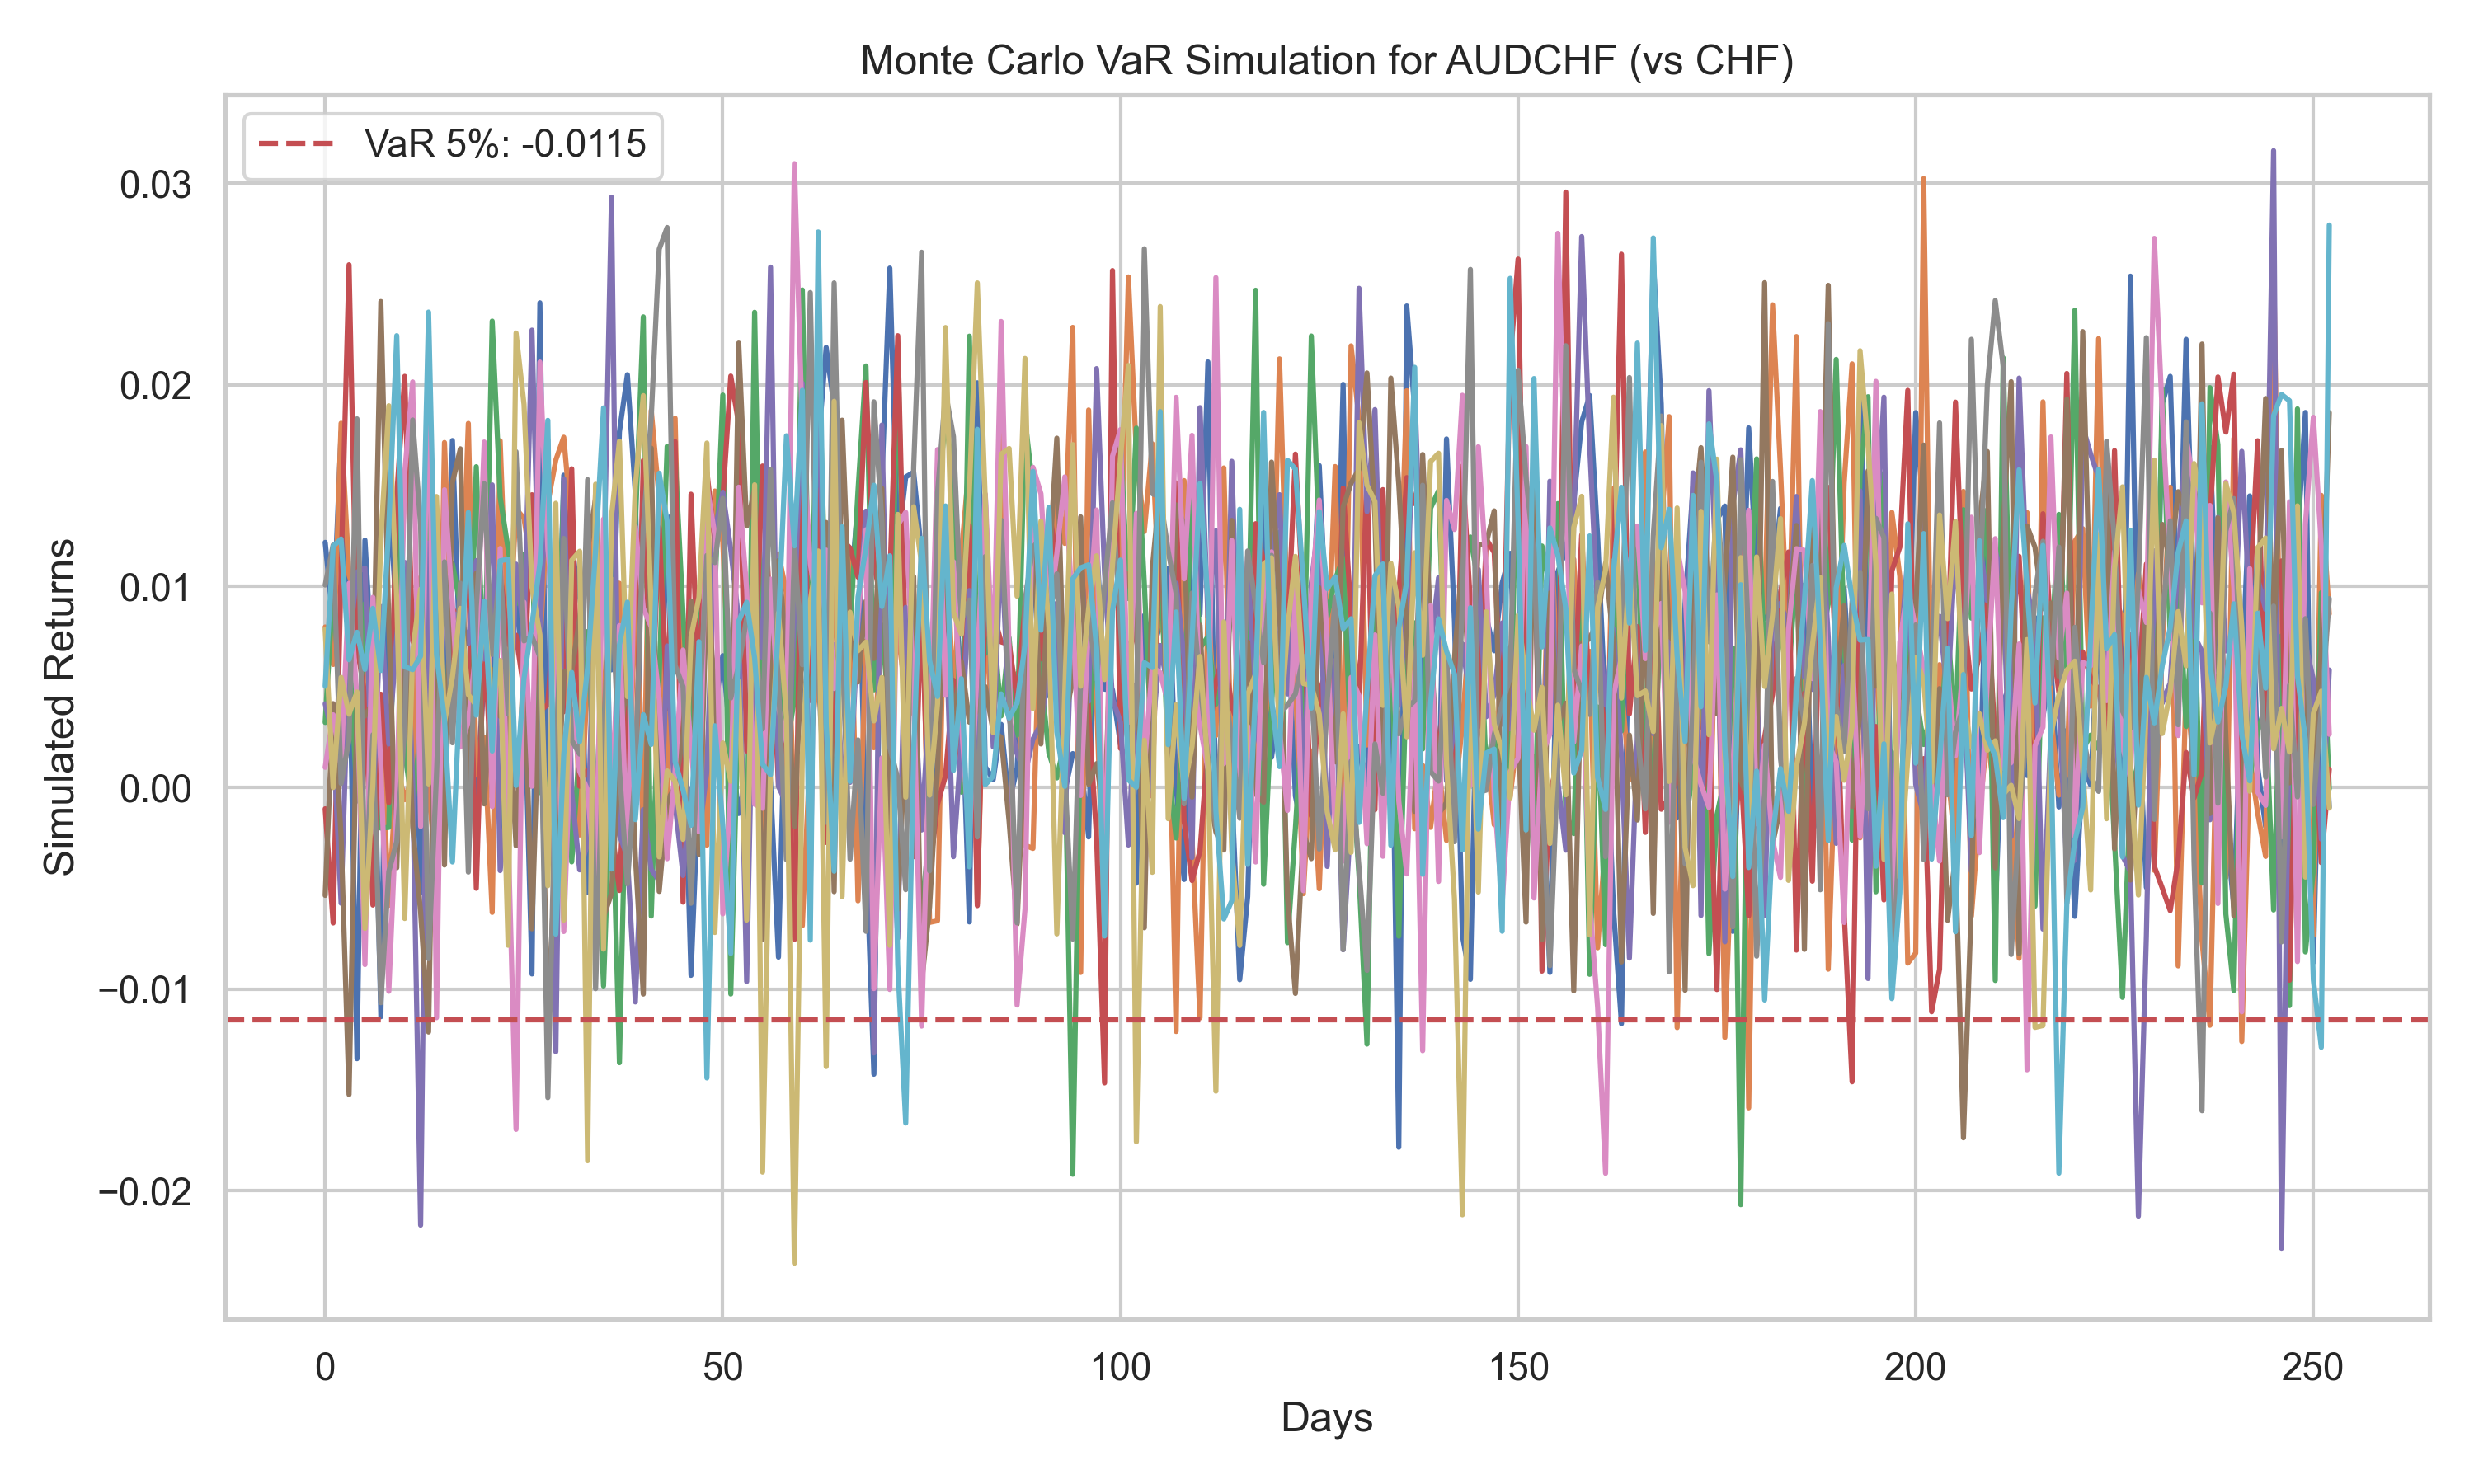
\includegraphics[width=0.48\linewidth]{reports/figures/monte_carlo_var_simulation_AUDCHF_vs_CHF.png}  \label{fig:monte_carlo_var_simulation_AUDCHF_vs_CHF}
    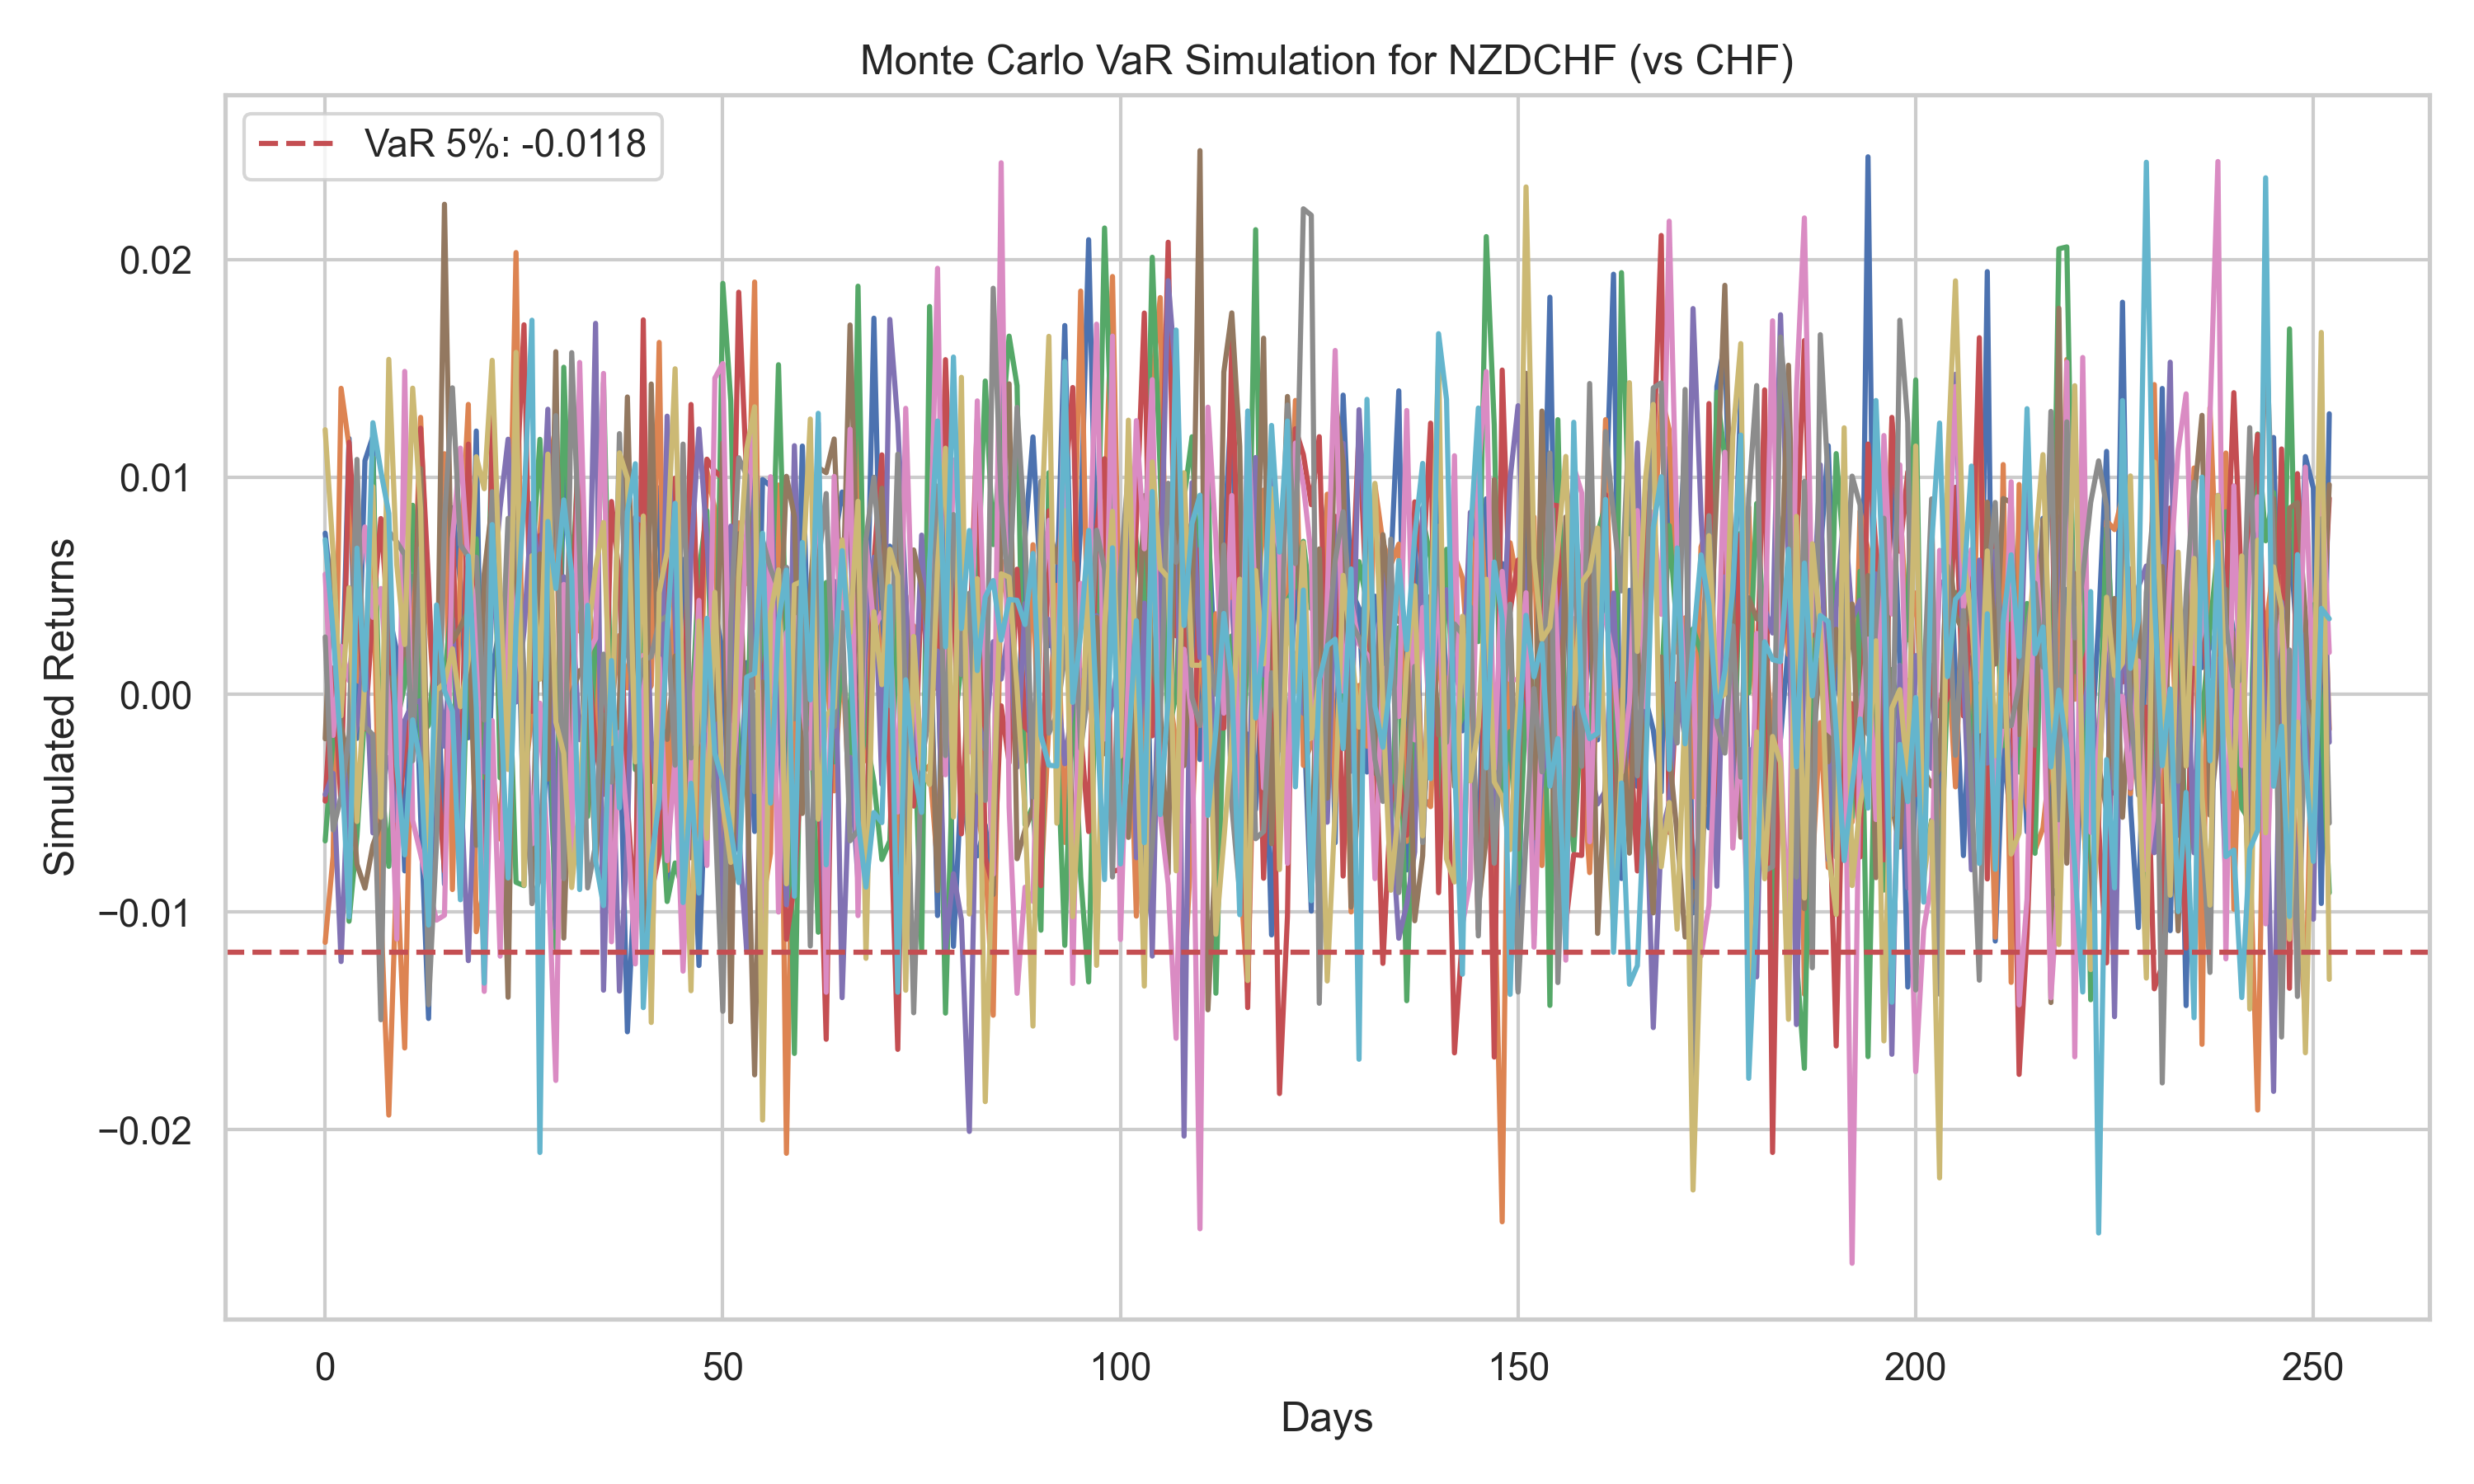
\includegraphics[width=0.48\linewidth]{reports/figures/monte_carlo_var_simulation_NZDCHF_vs_CHF.png}   \label{fig:monte_carlo_var_simulation_NZDCHF_vs_CHF}
    \caption{\footnotesize Monte Carlo VaR Simulation of AUDCHF vs. CHF (left) and NZDCHF vs. CHF (right)}  
\end{figure}
\end{frame}
% ---------------------------------------------------------------------------
\begin{frame}
\frametitle{Main Findings}
\framesubtitle{VaR Calculation}
\begin{itemize}
    \item AUD \& NZD carry sustained risk characteristics, and investors should be particularly cautious when considering these currency pairs.
    \item SEK shows increased risk in
    the Monte Carlo simulation. SEK may face greater uncertainty and potential risks in future market volatility.
\end{itemize}
\end{frame}
% ---------------------------------------------------------------------------
\begin{frame}
\frametitle{Main Findings}
\framesubtitle{Price Simulation}
GBP shows the most significant price volatility = 0.4, with high future price uncertainty.
\begin{figure}[h]
    \centering  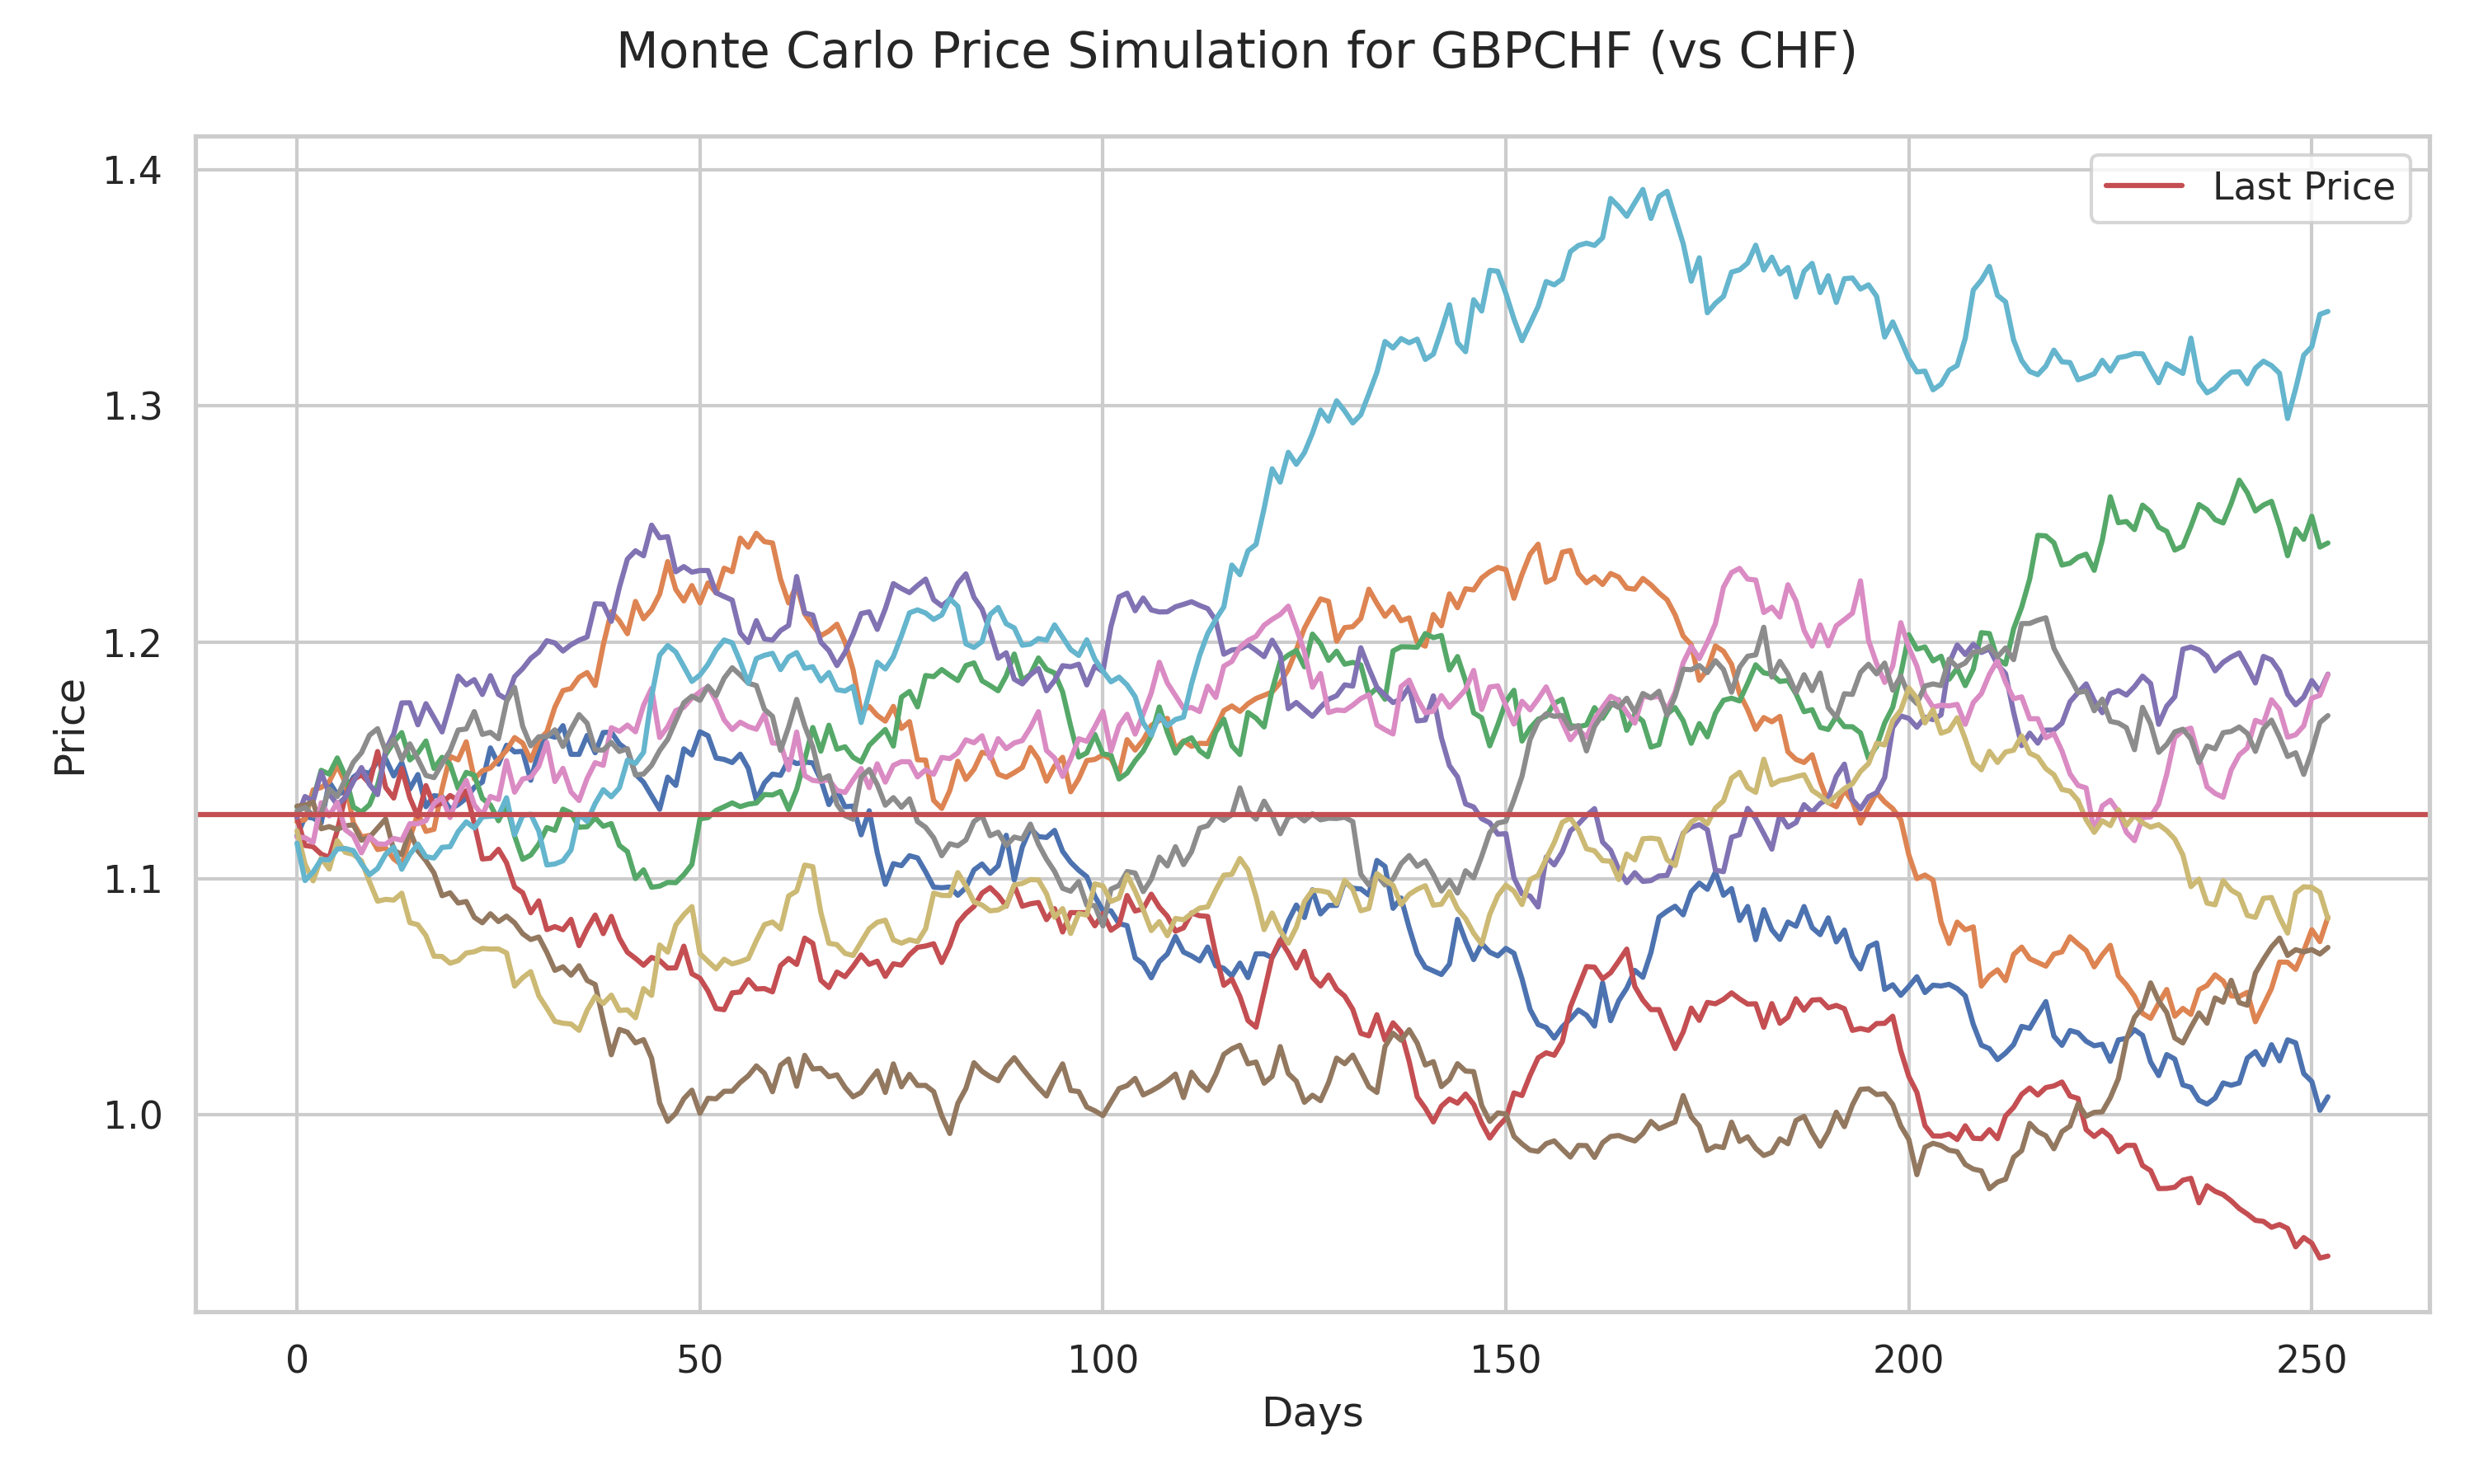
\includegraphics[width=0.75\linewidth]{reports/figures/monte_carlo_price_simulation_GBPCHF_vs_CHF.png}
    \caption{Monte Carlo Price Simulation of GBPCHF vs. CHF}  \label{fig:monte_carlo_price_simulation_GBPCHF_vs_CHF}
\end{figure}
\end{frame}
% ---------------------------------------------------------------------------
\begin{frame}
\frametitle{Main Findings}
\framesubtitle{Price Simulation}
Volatility of AUDCHF is around 0.33, and of NZDCHF is 0.27, also reflecting considerable price uncertainty.
\begin{figure}[h]
    \centering
    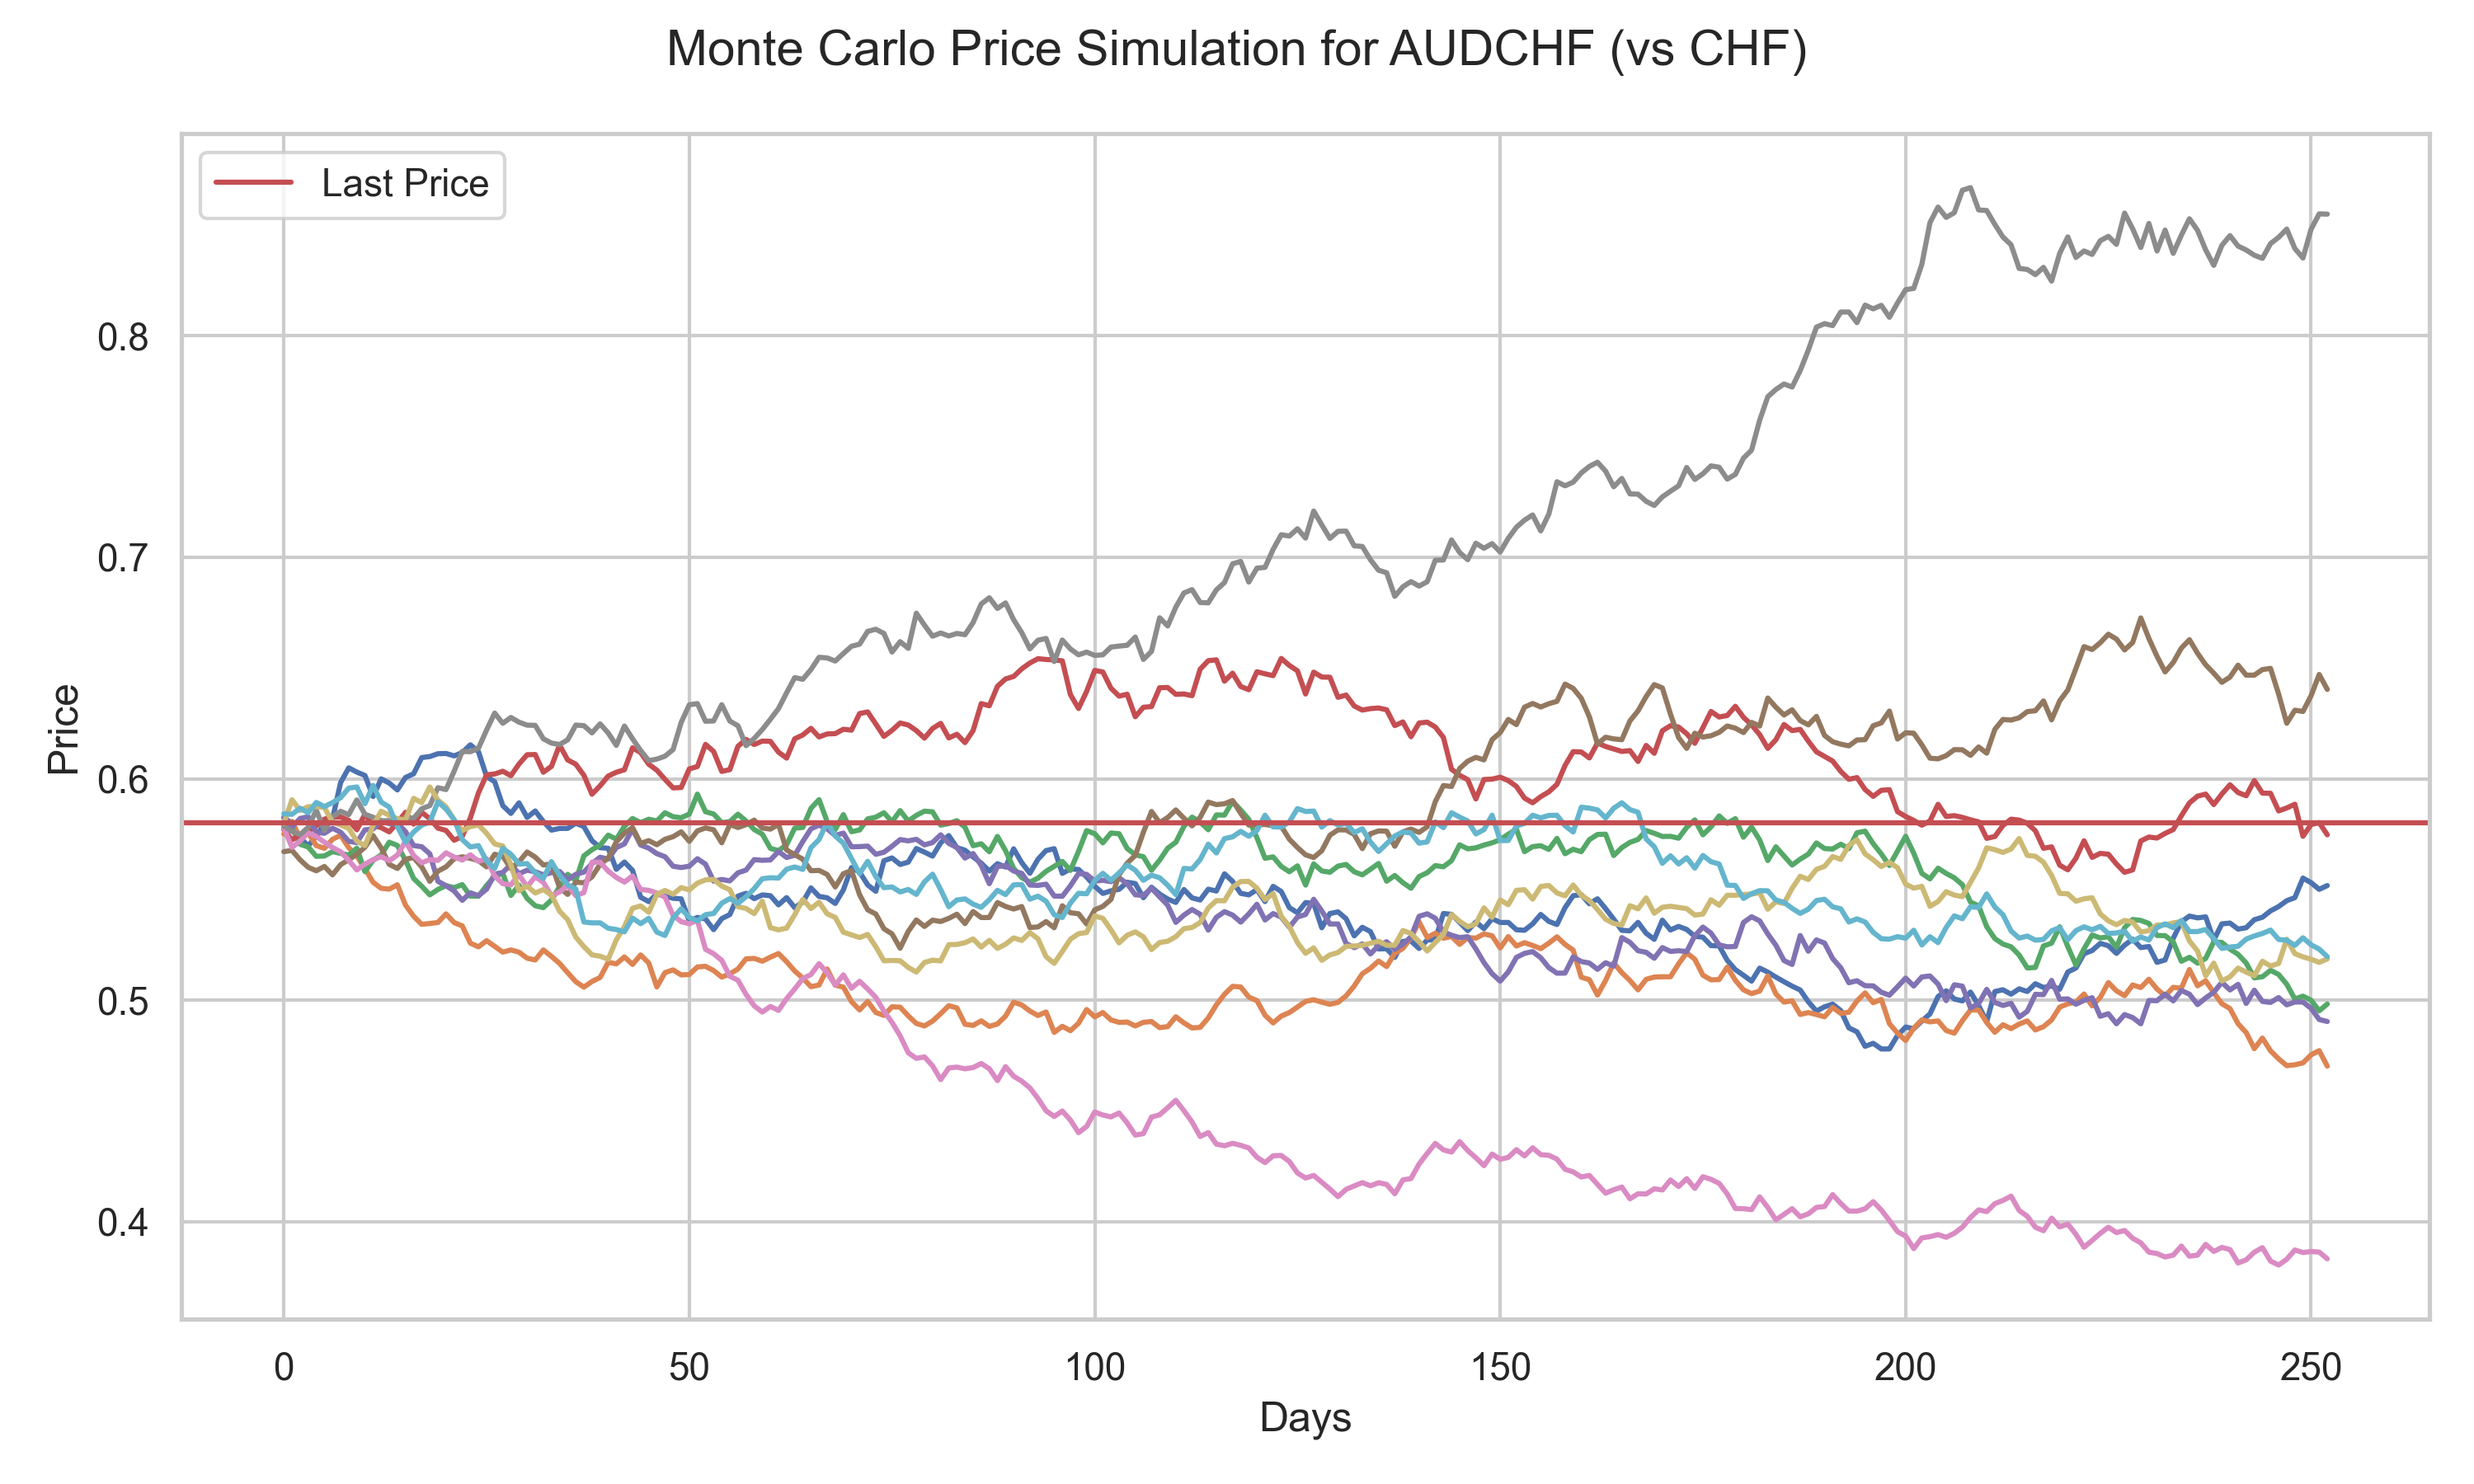
\includegraphics[width=0.48\linewidth]{reports/figures/monte_carlo_price_simulation_AUDCHF_vs_CHF.png}    \label{fig:monte_carlo_price_simulation_AUDCHF_vs_CHF}
    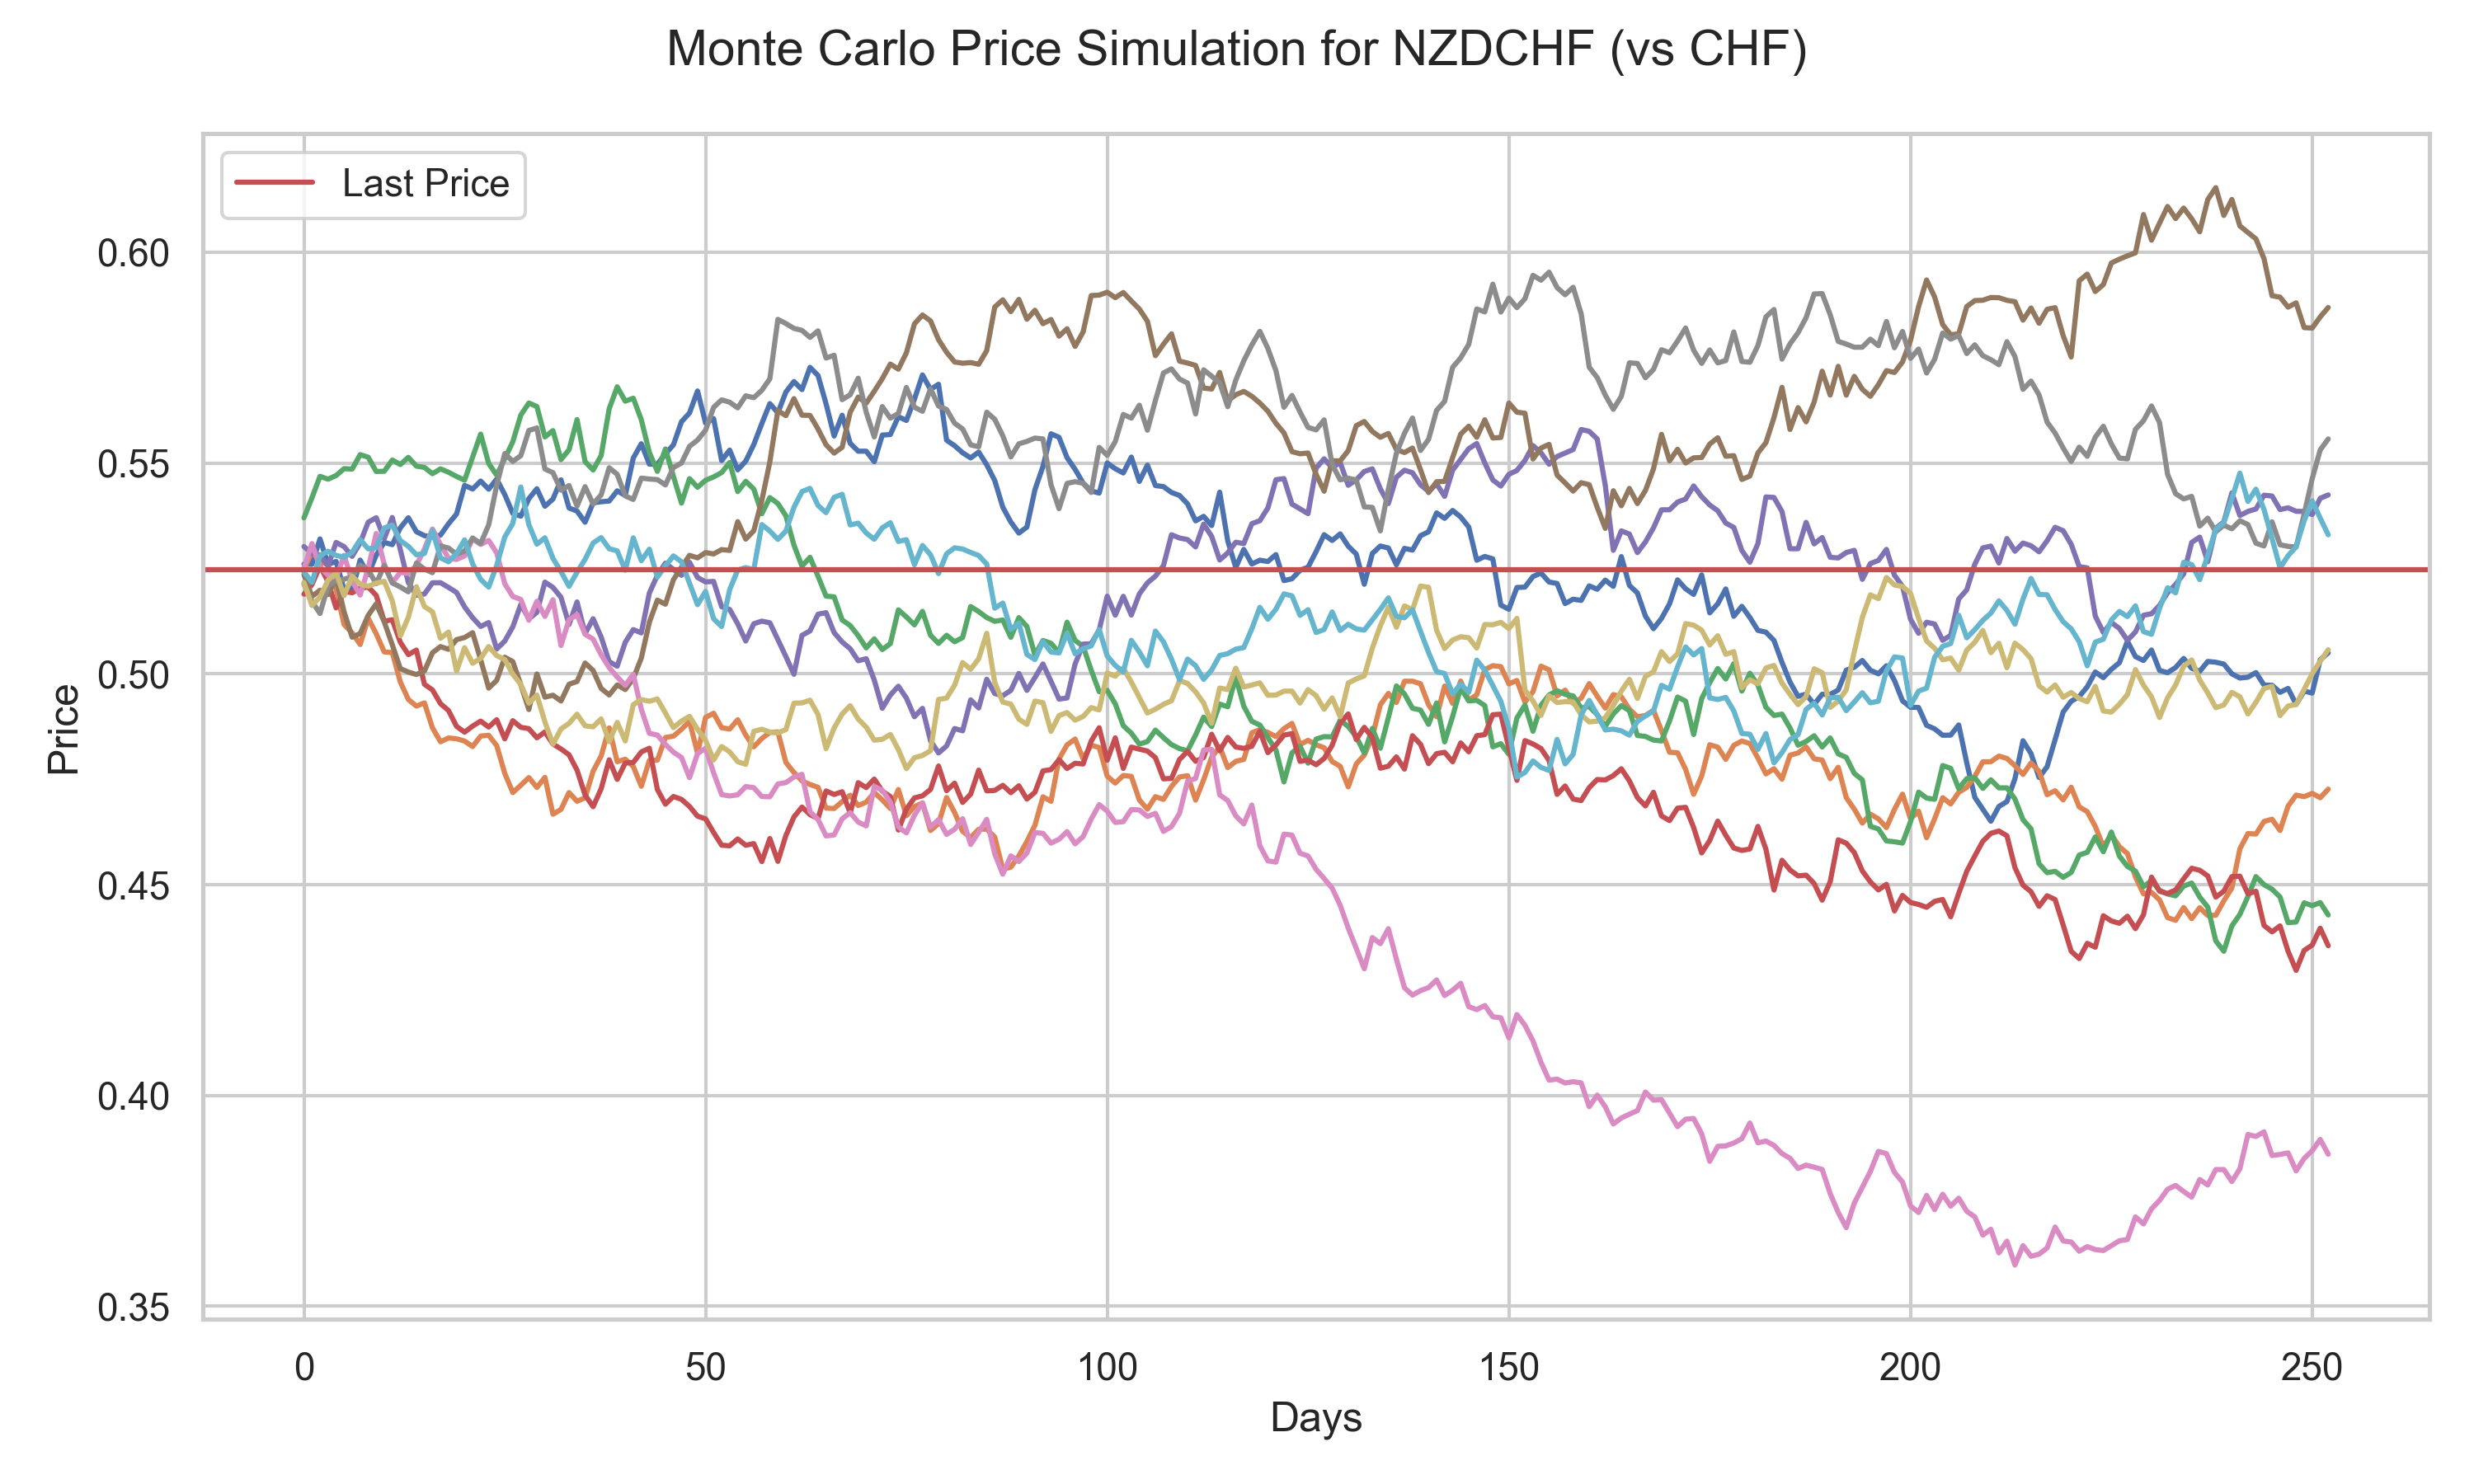
\includegraphics[width=0.48\linewidth]{reports/figures/monte_carlo_price_simulation_NZDCHF_vs_CHF.png}  \label{fig:monte_carlo_price_simulation_NZDCHF_vs_CHF}
    \caption{Monte Carlo Price Simulation of AUDCHF vs. CHF (left) and NZDCHF vs. CHF (right)} 
\end{figure}
\end{frame}
% ---------------------------------------------------------------------------
\begin{frame}
\frametitle{Main Findings}
\framesubtitle{Price Simulation}
For \textbf{both VaR and price simulations}:
\begin{itemize}
    \item AUD and NZD are high-risk and high-reward currency pairs, suitable only for investors willing to take substantial risks.
    \item Despite GBP has a relatively low VaR, but price volatility of 0.4 indicates strong future price fluctuations. Investors fully consider the risks associated with its price movements.
\end{itemize}
\end{frame}
% ---------------------------------------------------------------------------
\begin{frame}
\frametitle{Main Findings}
\framesubtitle{Price Simulation}
\begin{itemize}
    \item JPY has the lowest price volatility 0.0022, indicating extremely low future price fluctuations. 
    \item The Monte Carlo simulation result consistently remaining around 0.9\%. JPY demonstrates very \textbf{stable} risk characteristics. 
\end{itemize}
\begin{figure}
    \centering  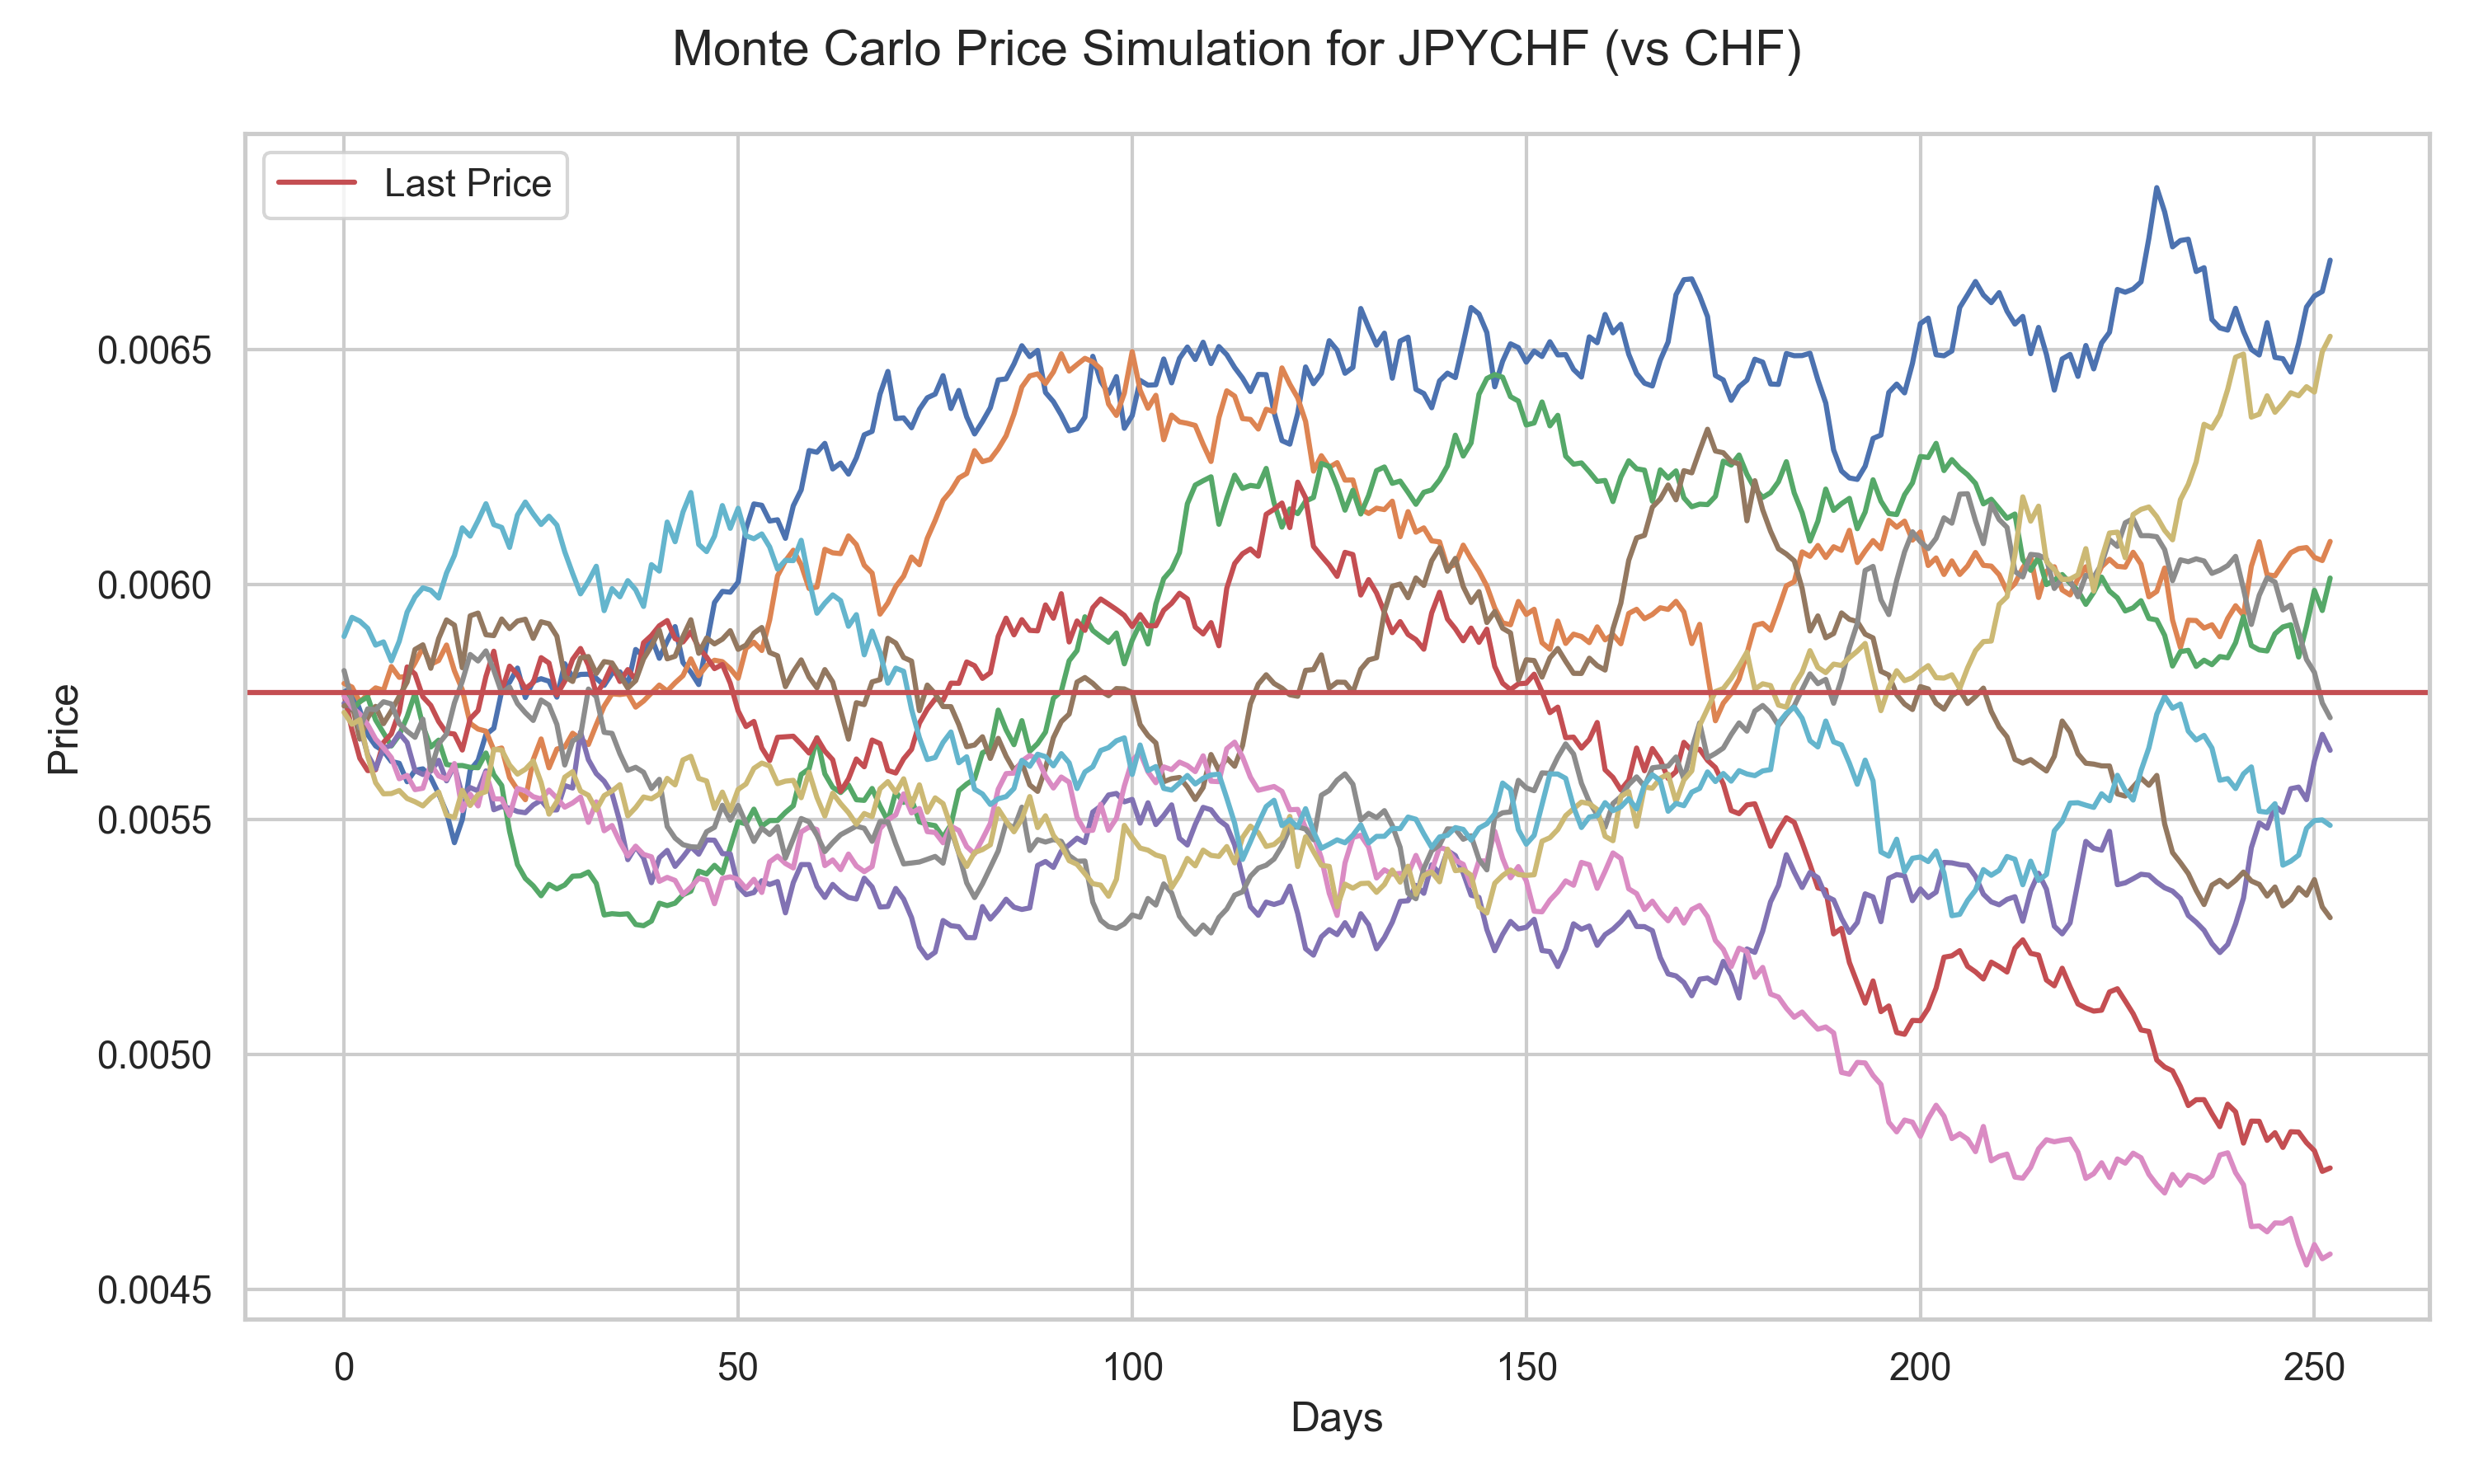
\includegraphics[width=0.48\linewidth]{reports/figures/monte_carlo_price_simulation_JPYCHF_vs_CHF.png}  \label{fig:monte_carlo_price_simulation_JPYCHF_vs_CHF}
    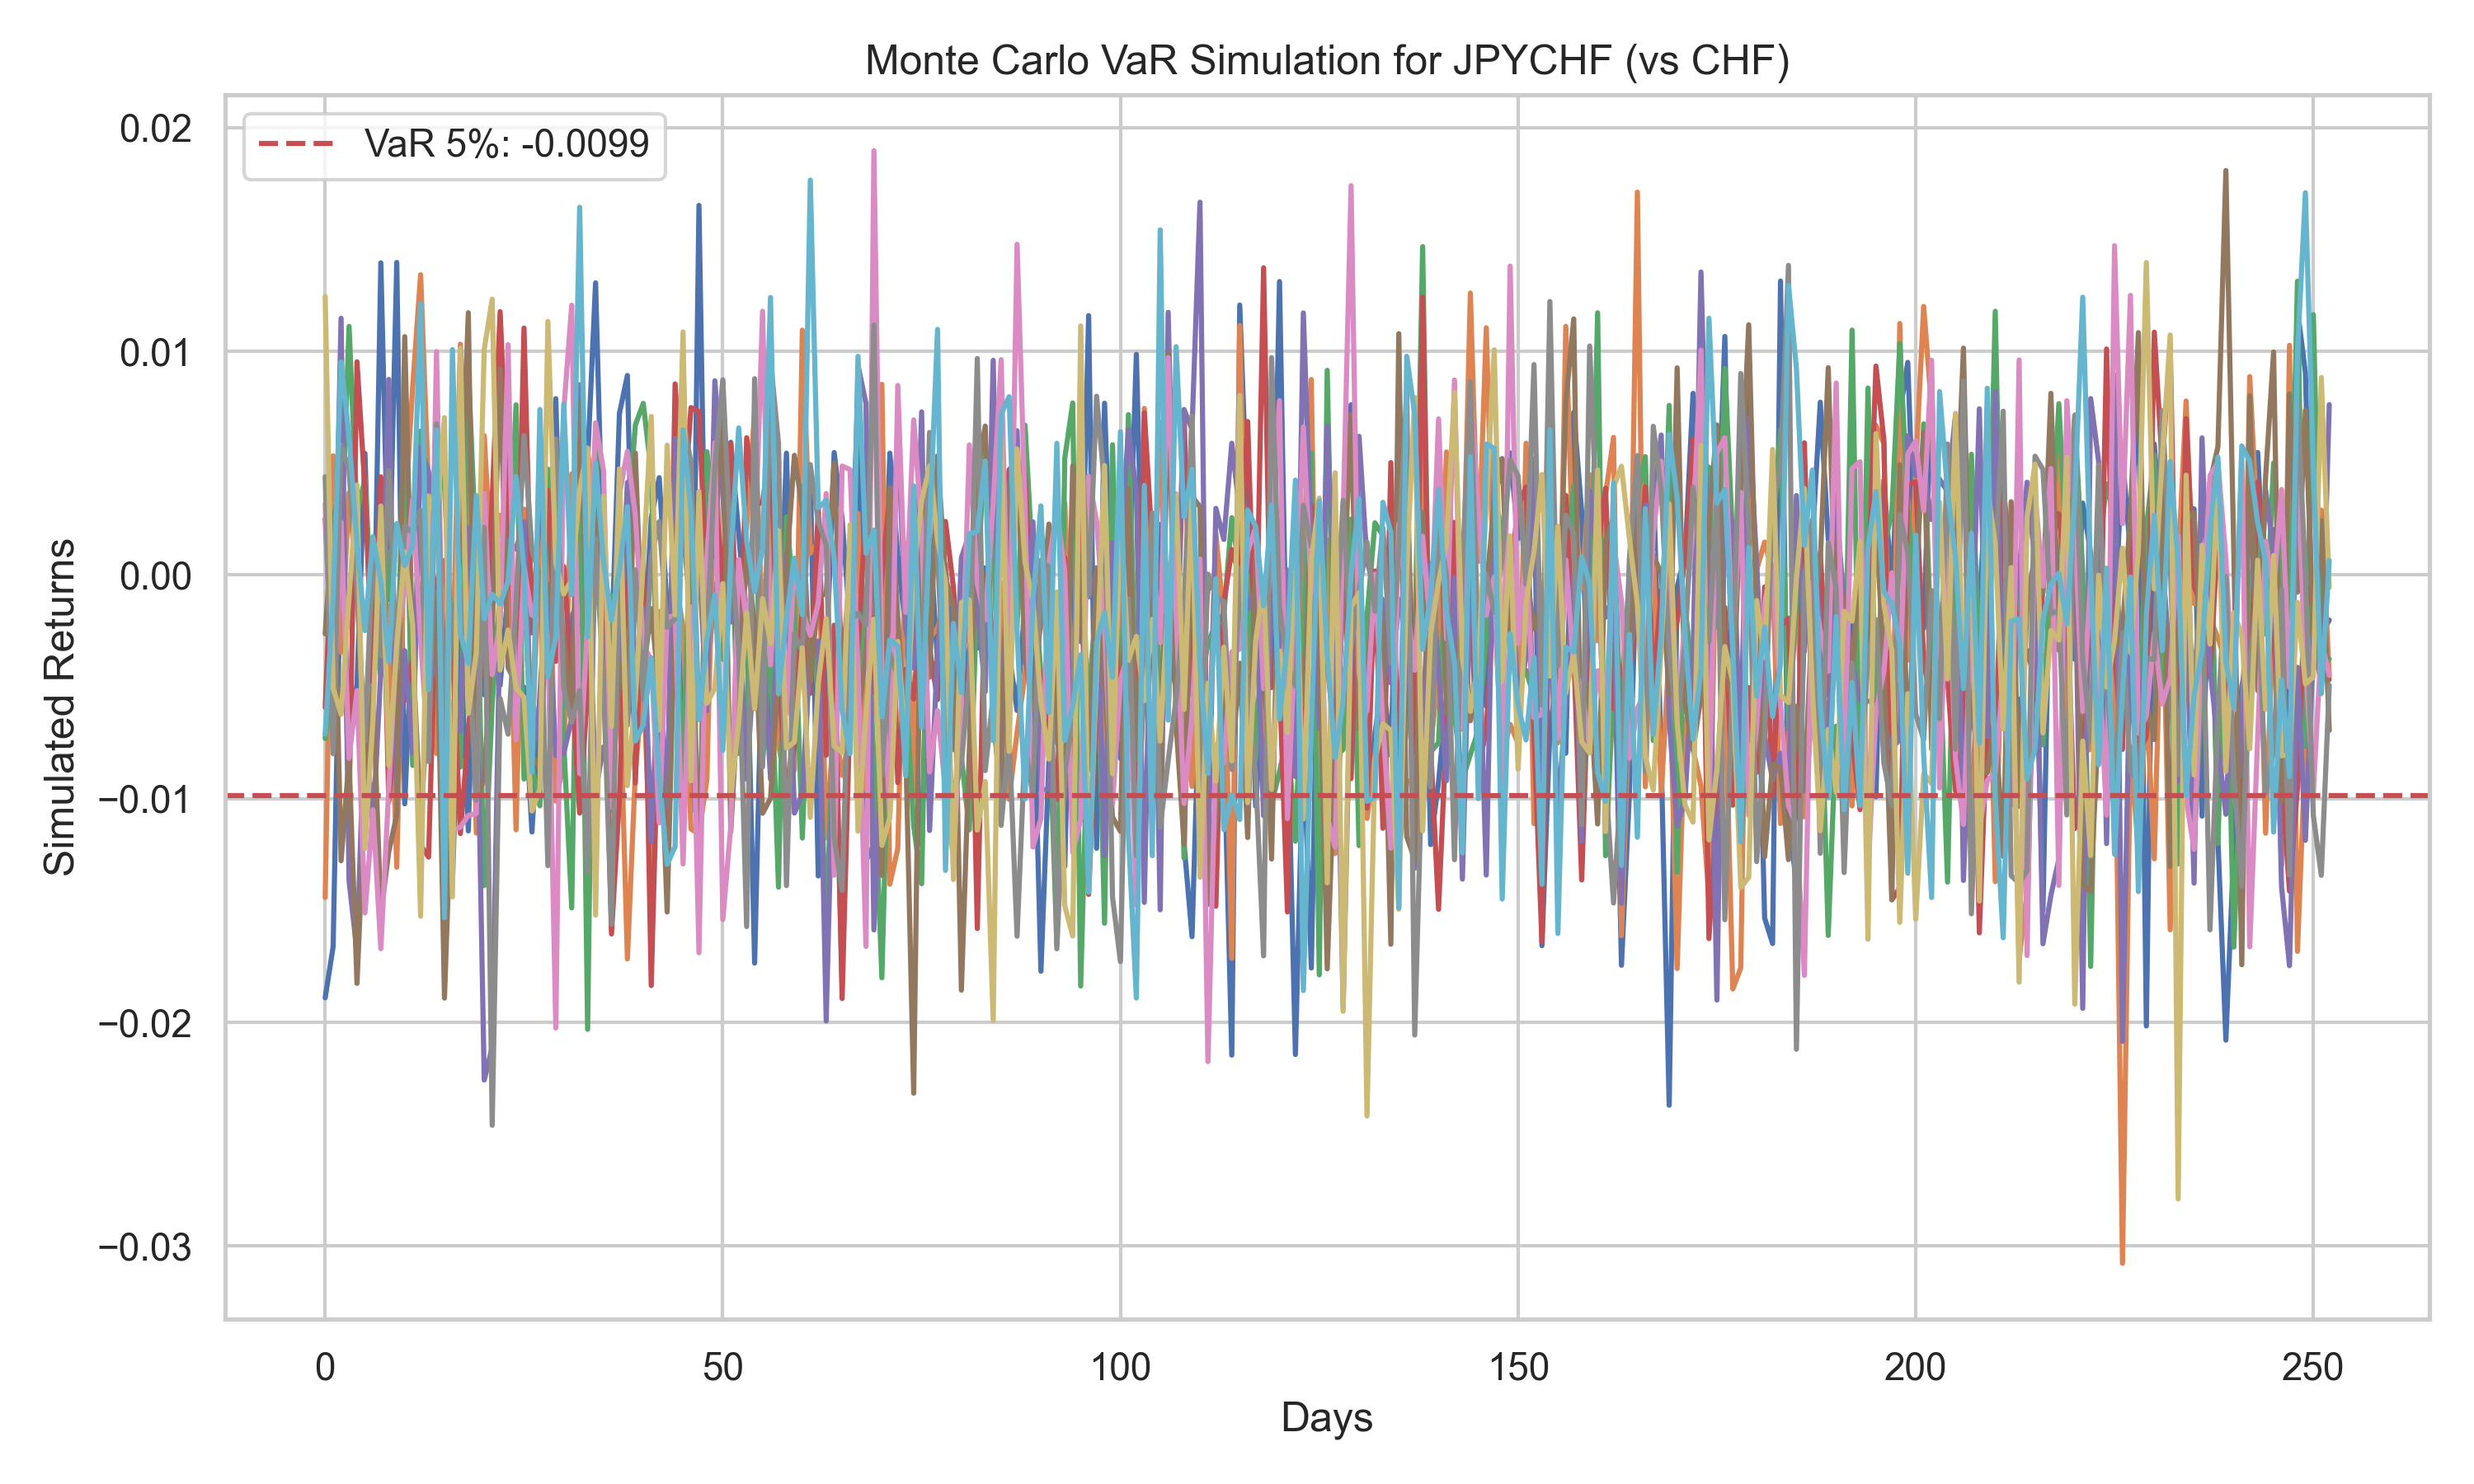
\includegraphics[width=0.48\linewidth]{reports/figures/monte_carlo_var_simulation_JPYCHF_vs_CHF.png}  \label{fig:monte_carlo_var_simulation_JPYCHF_vs_CHF}
    \caption{\footnotesize Monte Carlo price siulation (left) and VaR simulation (right) for JPY-CHF.}
\end{figure}
\end{frame}
% ---------------------------------------------------------------------------
\begin{frame}
\frametitle{Main Findings}
\framesubtitle{Price Simulation}
Low volatility and steady VaR make JPY an excellent hedging option in an investment portfolio, especially suitable for investors seeking lower-risk investments.
\end{frame}
% ---------------------------------------------------------------------------
\begin{frame}
\frametitle{Main Findings}
\framesubtitle{Regression Analysis}
The return rate of JPY fluctuates significantly with changes in interest rates, with $\beta = -3.25$ and highly significant.
\begin{table}[h]
\centering
\caption{\footnotesize Regression summaries of exchange rate returns on interest rate differentials.} 
\label{tab:var_results}
\resizebox{\textwidth}{!}{
\pgfplotstabletypeset[
    col sep=comma,
    string type,
    columns={Country, Alpha, Beta, Alpha Std.Err., Beta Std.Err., Alpha t, Beta t, Alpha P>|t|, Beta P>|t|},
    columns/Country/.style={string type, column name=Country},
    columns/Alpha/.style={fixed, precision=4, column name=$\alpha$},
    columns/Beta/.style={fixed, precision=4, column name=$\beta$},
    columns/Alpha Std.Err./.style={fixed, precision=4, column name=std.err\_$\alpha$},
    columns/Beta Std.Err./.style={fixed, precision=4, column name=std.err\_$\beta$},
    columns/Alpha t/.style={fixed, precision=4, column name=t-value\_$\alpha$},
    columns/Beta t/.style={fixed, precision=4, column name=t-value\_$\beta$},
    columns/Alpha P>|t|/.style={fixed, precision=4, column name=p-value\_$\alpha$},
    columns/Beta P>|t|/.style={fixed, precision=4, column name=p-value\_$\beta$},
    every head row/.style={before row=\hline, after row=\hline},
    every last row/.style={after row=\hline}
]{reports/figures/regression_summaries.csv}
}
\end{table}
Due to the stability of the Japanese economy, the overall volatility of the yen is controlled by certain factors that may reduce its extreme short-term risk.
\end{frame}
% ---------------------------------------------------------------------------
\begin{frame}
\frametitle{Main Findings}
\framesubtitle{Regression Analysis}
Regression results for NZD ($\beta$ = 0.13, and not significant) implies that interest rate changes do not have a major impact on NZD in the regression model. 

As previous, NZD has considerable volatility in the actual market, then there may be other factors significantly affect NZD, e.g. commodity price fluctuations (as New Zealand is a major commodity exporter~\cite{blundell1990exchange}) and speculative behavior in the foreign exchange market.
\end{frame}
% ---------------------------------------------------------------------------
\begin{frame}
\section{Conclusion}
\frametitle{Conclusion}

\end{frame}
% ---------------------------------------------------------------------------
\begin{frame}
\section{References}
\frametitle{References}
\printbibliography
\end{frame}
% ---------------------------------------------------------------------------

\end{document}
